\documentclass[11pt]{article}
\usepackage{mypackages}
\begin{document}

\maketitle

\subsection{Using deep learning for approximating functions}

In the last section we claimed that a neural network could be used to approximate the
state-value and action-value functions.
When we refer to a neural network, what we mean is an artificial neural network -
a computational model that emulates connections between neurons in the human brain.
Formally this means that we wish to find the functions $v_\pi^{\sim}(s)$ and $q_\pi^{\sim}(s,a)$ that
satisfies $v_\pi^{\sim}(s) \approx v_\pi(s)$ and $q_\pi^{\sim}(s,a) \approx q_\pi(s, a)$.
In general this means that for a function $f(x)$, the neural network tries to approximate
$f^{\sim}(x)$ such that $f^{\sim}(x)$ varies the least from $f(x)$ for all $x$ in the input
space\cite{DeepLearningBook}.
It does so by adjusting its parameters based on experience - data for which $f(x)$ is already known -
that it can use to compute how well the current approximation is performing.

This data is exactly what is available to us in the agent-environtment model, when there is a natural terminal state,
since we can then use the experienced actual returns to update the weights of the models.

\subsubsection{Layers, neurons and connections}

The goal of deep learning is to separate difficult problems into smaller and simpler problems
and in this process create a hierarchy of concepts, where each concept can be described in terms
of simpler concepts\cite{DeepLearningBook}.

In other words a neural network consists of layers that each represent a concept, which
when connected are able to solve the complex problem at hand.
With this definition of a neural network the approximation function $f^{\sim}(x)$ can be
defined as
\begin{equation}
    f^{\sim}(x) = f^{k}(f^{k-1}( \cdots f^{0}(x) \cdots))
\end{equation}
for a network with $k$ \textit{layers}.
The only layers that have their dimensions restrained are the first and last, since they are defined by the
dimensions of the input and the output of the approximator function.
Since we won't be seeing the output of the layers in between we call them \textbf{hidden layers}.

Each layer consists of a number of \textit{neurons} that are connected to the neurons of the
next layer.
%%%% Figure of layers
\begin{figure}[!h]
    \centering
    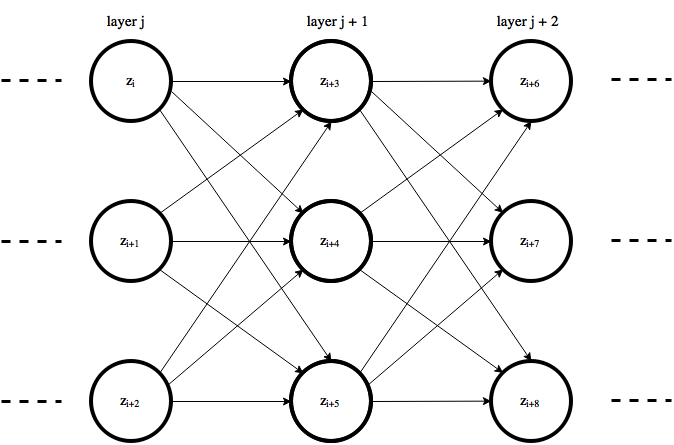
\includegraphics{include/layers.png}
    \caption{A series of layers in a fully connected neural network.}
    \label{fig:layers}
\end{figure}
When we discuss layers in this project we will only be referring to \textit{dense}
layers where every neuron is connected to all neurons in the subsequent layer - a fully
connected neural network.
The reason for this choice is that \textit{sparse} neural networks, where every neuron is not
connected to every neuron of the following layer, can be 'emulated' by a dense network by setting some of the
weights to 0.

Each neuron transforms its series of input signals into a single output signal which is then sent to
each neuron in the following layer through a \textit{weighted connection}, where
the weight of the connections define the importance of the signals.
%%%% A drawing of a neuron “up close”
\begin{figure}[!h]
    \centering
    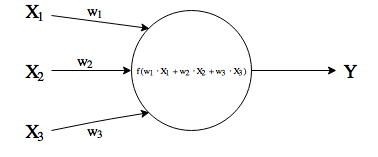
\includegraphics{include/neuron.png}
    \caption{The structure of a single neuron.}
    \label{fig:neuron}
\end{figure}
Thus the hidden layers aim to extract the key features of the original input.
The input of the neuron typically goes through a function which aims to activate
a property of the input.
%% Introduce activators


The idea in an Artificial Neural Network is that we building a network of \textit{neurons} which is connected to each other,
and the learning is done by adjusting the connection between these neurons,
the connection parameter between two neurons is called \textit{weights} and by adjusting these weights
we can optimize the network for solving a problem.

\subsubsection{Updating the weights using gradients}


\end{document}
